\documentclass[11pt]{article}
\usepackage[margin=0.7in]{geometry}
\usepackage{amsmath,amssymb,graphicx,xurl,hyperref,array}
\setlength{\parindent}{0pt}\setlength{\parskip}{4pt}
\setlength{\emergencystretch}{3em}
\begin{document}
{\Large Lossless projection of the unfinished m5 norm input}\par
2026-11-13. Source\path{ccd9e23f1}. Unsigned evidence [pcc:unverified].

The actual23-variable,25-equation RR input reduces to four function
coefficients. The other19 variables are uniquely recovered by target
completion and monic polynomial division. Native symbolic substitution checks
all original equations:20 vanish identically, the last5 are exactly the
reduced membership constraints. This is a lossless representation trade,
not a measured solver gain [pcc:unverified].

\begin{center}
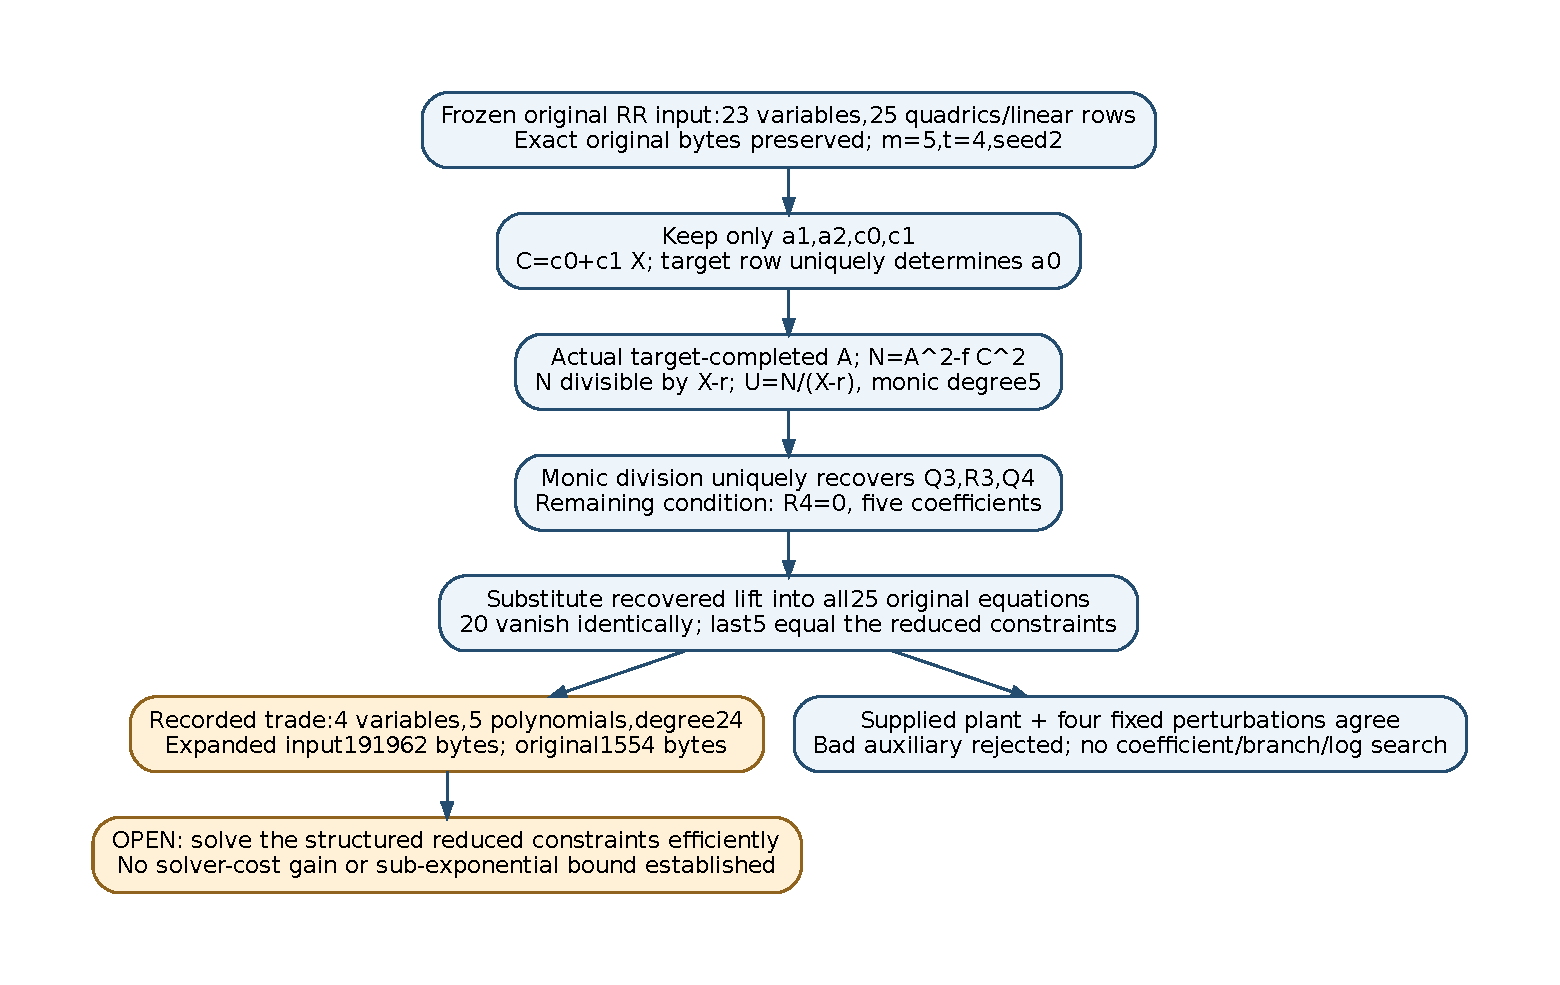
\includegraphics[width=0.96\linewidth,height=0.55\textheight,keepaspectratio]{projection.pdf}
\end{center}

For $C=c_0+c_1X$, $D=X^3+a_2X^2+a_1X$, set
\[
 a_0=zC(r)-D(r),\quad A=D+a_0,\quad
 N=A^2-fC^2,\quad U=N\mathbin{\mathrm{div}}(X-r).
\]
The actual target satisfies$z^2=f(r)$; the norm division is exact and
$U$ is monic degree5. No variable denominator or new saturation/chart
guard discards old algebraic solutions. The universal Lean model and
concrete native compiler binding are separate evidence scopes
[pcc:unverified].

Unsigned claims: canonical quotient\path{PCC-20261113-c1ec0b}; terminal
membership\path{PCC-20261113-a3e4cb}; native binding\path{PCC-20261113-b465d8}.

\newpage
{\Large Exact controls and the degree/input trade}\par
The copied Dickson m5,t4,seed2 fixture has$p=14680063$,
$f=X^3+3607823X+6826282$, target$(r,z)=(5400989,8855456)$,
terminal$c=12691281$. Original input SHA256:\par
\path{9ba376d81c05109b11102c645153f9204df233600fec5851993a6bd5787e3cff}.
Exact original bytes and historical paths remain intact [pcc:unverified].

Let$D_0=X$, $D_{j+1}=D_j^2-2$. Compute the actual divisions
\[
 D_3=UQ_3+R_3,\qquad R_3^2-2-c=UQ_4+R_4.
\]
Only the five coefficients of$R_4$ remain. The direct remainder
$(D_4-c)\bmod U$ equals$R_4$. Every one of the25 original source equations
is parsed independently and substituted into exact four-variable sparse
polynomials. The first20 become zero polynomials; the last5 equal those
five residuals coefficient by coefficient [pcc:unverified].

\begin{center}\small
\begin{tabular}{rrr}
Reduced$X$ coefficient & Total degree & Terms\\\hline
4&24&1103\\3&24&1445\\2&24&1830\\1&24&2171\\0&24&2366
\end{tabular}
\end{center}
The expanded reduced input is191962 bytes; the original is1554 bytes.
Both full inputs are retained. The generator records682901 sparse
coefficient-pair products and peak2366 observed terms below the finite
guards. These are construction counts, not a solver cost model or timing.
The one write-once artifact exits0 under256MiB/120 CPU-second caps
[pcc:unverified].

The five prospectively fixed assignments are the supplied plant plus one
increment of each core coordinate. The plant recovers all23 supplied values
and all25 residuals vanish. Each perturbation preserves the20 identically
zero rows, matches the reduced five residuals exactly and is nonzero in this
fixture. Corrupting the recovered Q3 leading coefficient rejects. No search
for coefficients, branches, roots or logarithms; no Groebner solver or paid
job ran. Unit tests reuse these cases [pcc:unverified].

\textbf{Raw-source audit.} The earlier m5,t4 RR comparison never completed.
R2b timed out; R3 RR attempts were interrupted. RRa2's exact input hash
matches, its last log begins an unfinished464562-by390983 degree7 matrix,
and the raw CloudTrail object records BidEvictedEvent at11:09:30Z on Nov9.
The protocol grants no bounds from Spot-lost partial jobs. The object has
no pod/node field; that association relies on the historical assessment.
Idle-start msolve output and earlier close CPU/real pairs do not establish
continuous isolation or final-step timing. A reliable retry could decide
one cell, not an asymptotic growth law [pcc:unverified].

Source audit\path{PCC-20261113-08f893}; copied source paths, hashes, raw
metadata and explicit limits are in\path{sources-checked.json}.

\newpage
{\Large Universal model, actual source binding and next test}\par
Lean4.35.0.\par
CryptoLean \path{148f5dc389b341401e06d76abe7783c4ccf42f2e}.\par
Mathlib \path{cfc55fc58714a59dc06e6e79edc6d1d95140d3c2}.\par
Build004 passes16 new statements with only propext, Classical.choice and
Quot.sound. Current source gate exits0:286 statements,0 additional trusted.
The new module's import-inclusive fresh replay76692 exits0.
Native tests002 pass3, strict clippy002 and release build pass. Failed
attempts remain. All scientific claims are unsigned; default-PATH PCC
checks remain source-only not\_covered [pcc:unverified].

\begin{center}\footnotesize
\begin{tabular}{p{0.38\linewidth}p{0.55\linewidth}}
NormMembershipElimination & Exact statement scope\\\hline
completionRow / completionUnique & Actual constant completion; target row and uniqueness\\
normAtTarget / canonicalNormQuotient & Actual target/curve equations; norm zero and exact computed quotient\\
normQuotientUnique / divisionUnique & Actual monic factor, quotient and bounded remainder are determined\\
reducedStep / reducedMaster & Actual modular tower equals direct master remainder\\
canonicalTowerLift / canonicalTowerBound & Actual computed auxiliaries exist with the degree guard\\
towerUnique & Every bounded old tower equals the computed one\\
terminalMembership & Nontrivial ring, positive-degree monic modulus; terminal iff divisibility\\
normWindow / supportWindow & Field, monic cubic$A$, cubic$f$, $\deg B\le1$; norm/support monic degrees6/5\\
completionWindow / quotientWindow & Completion preserves degree3; quotient degree$\le3$
\end{tabular}
\end{center}
The model does not assume successful old auxiliaries to construct the new
ones. Its universal monic-division facts are distinct from the native
normal-form binding of all25 literal expressions. No native comparison is
presented as a Lean-verified compiler [pcc:unverified].

Literal certificate\path{IDC1hb49f2953ff1e646f}, attestation
\path{PCC-20261113-5e61c7}, covers only$(D+ZB-D)^2-Z^2B^2=0$.
The unchanged canonical checker accepts32+16 replay points over its v1
fixed modulus. It does not encode monic division or the full projection;
the Lean pointer is separate. Its driver builds, but strict clippy retains
four existing style errors in unchanged canonical SHA256 under Rust1.99.1,
without suppression or checker edits [pcc:unverified].

\textbf{Sources checked.} KB MCP/executable unavailable. Read named public
repo sources and raw records, PKC2016 sections3.1--3.5/4.1/Table4,
Cheng cs0507026 Lemma3 and Caminata--Gorla2112.05579v2 section4.
Binary Nagao coefficient/block work is adjacent. Query token matches and
varying revisions do not establish exhaustive absence or novelty. Two
ePrint full texts returned403 and remain algorithmically unassessed
[pcc:unverified].

\textbf{Next discriminating action.} Compare a module-aware or circuit-preserving
solver on this exact projection with the strongest matched original system,
counting construction and every solving phase. Four variables and degree24
alone establish neither a gain nor a loss. No such solver/cost experiment
ran. The actual finder and complete$\exp(o(\log r))$ bit-cost bound remain
open; no benchmark/leaderboard/performance graph values change
[pcc:unverified].
\end{document}
